\subsection{MIDI Instrument}
\label{sec:midi_track}

A MIDI instrument track contains a sequence of MIDI events with its associated
instrument, including the synthesizer. This track is responsible for triggering the note on/off
events, pitch, velocity, etc. depending on the event scheduling as discussed in Section \ref{sec:sample_scheduling}.

\subsubsection{Choice of Instruments}

The oscillator-based synthesizer (Section \ref{sec:synthesizer}), Sfizz \cite{sfizz}, and FluidSynth \cite{fluidsynth} are chosen for playing instruments. 
Fluidsynth API provides support for Soundfont 2 (SF2) which are wavetable synths for storing myriads of sound samples. Which means these wavetable
synths can potentially mimick organic musical instruments for producing realistic music.

Soundfonts are used to store sampled instrument data, along with associated modulation and articulation parameters, 
as defined by the SoundFont Technical Specification \cite{soundfont_spec}. These pre-recorded samples makes it relatively cheaper to render
rather relying heavily on DSP algorithms. The same principle applies for SFZ, except that they heavily rely on WAV files 
with a plain-text containing a set of specifications in key/opcode pairs \cite{sfz_format}. 

\subsubsection{Class Structure Design}
The UML diagram (\Cref{fig:instrument_arch}) shows a complete UML diagram on how a class instance of the instrument track is designed.
The instrument utilizes the voices routed from either a synthesizer or Soundfonts using the APIs from FluidSynth and Sfizz. These 
APIs render and trigger a sample for each voice for as many times as the \texttt{generateSample()} function is called.

\begin{figure}[ht]
  \centering
  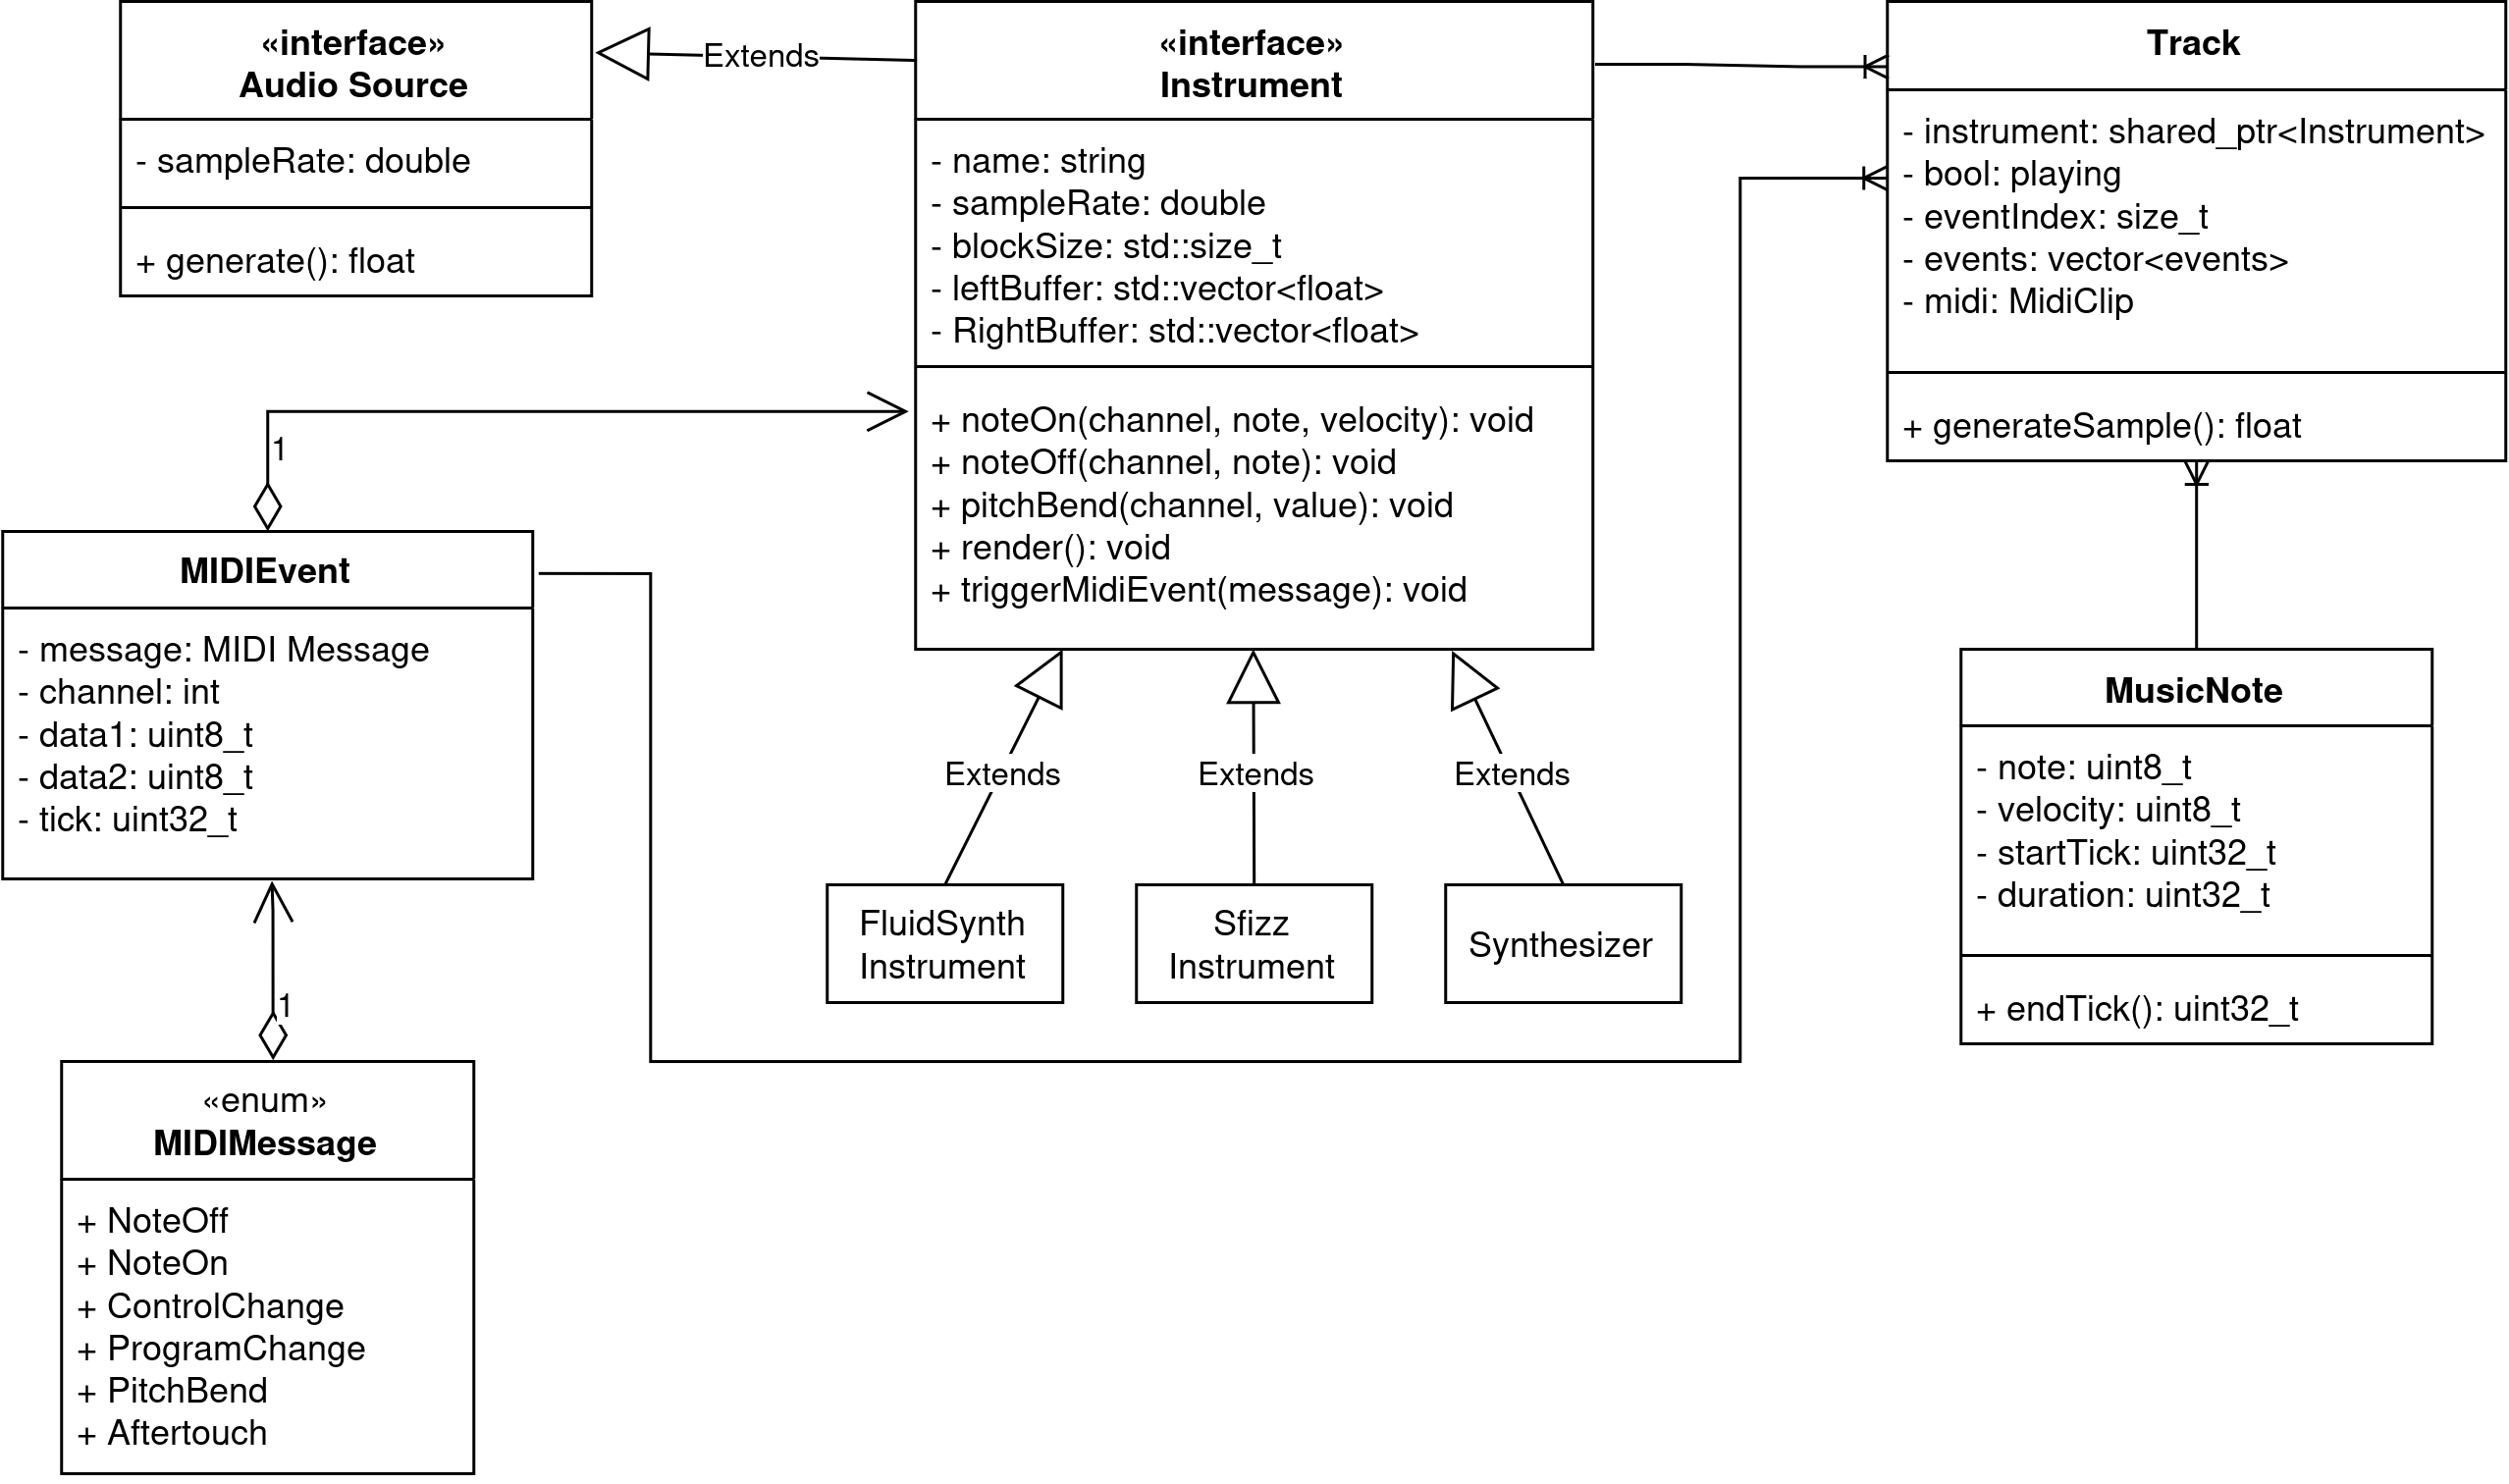
\includegraphics[width=\linewidth]{discussion/midi_instruments/figures/instrument_arch.png}
  \caption{UML Diagram describing the relationships between components of the track}
  \label{fig:instrument_arch}
\end{figure}


The list below provides a description for each of the entities/class structures:

\begin{enumerate}
    \item \textbf{Music Note}: Holds a pitch, velocity and channel number of a MIDI player
    \item \textbf{MIDI Clip}: Data Access Object (DAO) holding a collection of music notes, which is later on, converted to MIDI events
    \item \textbf{MIDI Message}: Provides a description on what the event must do (e.g. NoteOn, NoteOff, Pitch bend, etc.) \cite{midiassociation2015messages}
    \item \textbf{MIDI Event}: Specific action in the MIDI protocol to perform a specific task, with \texttt{data1} and \texttt{data2}
    as placeholders, depending on the MIDI Message
\end{enumerate}

\begin{quote}
NOTE: MIDI Channel segregates separate devices to allow a MIDI controller or sequencer to send different messages to each
of the devices.
\end{quote}

A MIDI event can be triggered from a DAO at a particular timestamp (see Section \ref{sec:sample_scheduling} on how it's done), 
or a MIDI input from an external input device. Once the program triggers the event, the MIDI message is sent 
to the instrument, which then triggers a function depending on the message determined by the \texttt{triggerMidiEvent(message)}.
It can trigger either \texttt{noteOn()} (plays a note), \texttt{noteOff()} (stops playing the note), or \texttt{pitchBend()} 
(deviates the pitch from the original) \cite{midiassociation2015messages}.

Notice that the track uses instrument as a shared pointer. Because the Instrument is an abstract class, and Fluidsynth and Sfizz is made to
inherit that class. Also an SF2 file can hold multiple instruments, therefore \texttt{std::shared\_ptr} allows multiple tracks to share
that FluidSynth instrument, provided that the tracks send messages with their own channel numbers (\Cref{prompt:inst_using_ptrs}) \cite{openai_chatgpt}.

\subsubsection{Rendering Mechanism}
Using these collection of events, the instrument renders samples which collectively creates sound. The program stores these samples
to its internal buffer (for both left and right channel) with its given \texttt{blockSize}. When a sample is sent to the audio engine 
using \texttt{generate()}, it takes the first sample from the buffer and then moves on to the next buffer. Eventually, the rendering 
process restarts when it reaches the end of the buffer. For e.g., if the block size is set to 512, and when the \texttt{Instrument} class
reaches the 513\textsuperscript{th} sample using generation, the \texttt{render()} method refills the buffer with the next 512 samples.
It is developed like this, because FluidSynth and Sfizz APIs only sends out blocks of samples by design 
(\Cref{prompt:render_block_reason}) \cite{openai_chatgpt}.

The rendering codes are provided in \Cref{app:fs_sfz_render}, Listing \ref{lst:sfz_render} and \ref{lst:fs_render}.